\documentclass{article}
\usepackage{graphicx} % Required for inserting images
\usepackage[utf8]{inputenc} % UTF-8 encoding
\usepackage[spanish]{babel} % Spanish language support
\usepackage{hyperref} % For clickable links in TOC
\usepackage{geometry} % For page margins
\usepackage{float} % For better figure placement
\usepackage{amsmath} % For mathematical equations
\usepackage{amsfonts} % For mathematical fonts
\usepackage{xcolor}
\usepackage{hyperref}
\hypersetup{
    colorlinks,
    linkcolor={blue!50!black},
    citecolor={red!50!black},
    urlcolor={blue!80!black}
}


\geometry{margin=1in} % Set page margins

\title{Minería de Datos: Clasificación Binaria de Estrellas y Galaxias}
\author{Juan Pablo de Alba Tamayo}
\date{Junio 2025}

\begin{document}

% Primera página: Logo
\begin{figure}[H]
    \centering
    
\includegraphics[width=0.75\linewidth]{logo.png}
\end{figure}

\newpage

% Segunda página: Título
\maketitle

\newpage

% Tercera página: Índice
\tableofcontents

\newpage

% Cuarta página: Lista de figuras
\listoffigures

\newpage

% Contenido del documento
\section{Introducción}

La astronomía moderna se enfrenta al desafío de procesar y clasificar enormes volúmenes de datos provenientes de observaciones astronómicas. Con el uso de telescopios de gran tamaño y estudios de cielo profundo, la cantidad de objetos celestes detectados ha crecido exponencialmente, haciendo impractica la clasificación manual de cada uno de estos objetos. En este contexto, la diferenciación entre estrellas y galaxias representa uno de los problemas fundamentales de clasificación en astronomía, ya que estas dos clases de objetos constituyen la mayoría de las fuentes puntuales detectadas en los estudios fotométricos.

Este proyecto tiene como objetivo desarrollar un sistema de clasificación automática para distinguir entre estrellas y galaxias utilizando técnicas de aprendizaje automático aplicadas a datos fotométricos. Se implementará un modelo de Regresión Logística optimizado que aprovecha las características discriminativas más relevantes de los objetos astronómicos. El análisis incluirá la exploración de los datos, el preprocesamiento especializado para datos astronómicos, la selección de características óptimas y la optimización de hiperparámetros para maximizar la eficacia del modelo. La implementación completa del proyecto se encuentra disponible en un notebook interactivo \cite{colab_notebook}.


\section{Definición del Proyecto}
% Agregar contenido aquí

\subsection{Objetivo}

El objetivo principal de este proyecto es desarrollar un sistema de clasificación automática que permita distinguir eficientemente entre estrellas y galaxias utilizando técnicas de aprendizaje automático. Específicamente, se busca:

\begin{itemize}
    \item Implementar un modelo de Regresión Logística optimizado para la clasificación binaria de estrellas y galaxias.
    \item Realizar un análisis de los datos fotométricos disponibles, incluyendo la exploración de patrones, distribuciones y correlaciones entre variables.
    \item Aplicar técnicas de preprocesamiento de datos, como transformaciones logarítmicas y escalado robusto.
    \item Optimizar los hiperparámetros del modelo mediante técnicas de búsqueda aleatoria (RandomizedSearch) para maximizar su efectividad.
    \item Desarrollar un pipeline que proporcione una capacidad de generalización y precisión superior al 90\% en la clasificación de objetos astronómicos.
\end{itemize}

\subsection{Expectativas}

Se espera que al finalizar este proyecto se haya logrado:

\begin{itemize}
    \item Alcanzar una precisión de clasificación superior al 90\% en el conjunto de datos de prueba, aprovechando la naturaleza bien diferenciada de las características entre estrellas y galaxias.
    \item Demostrar que la Regresión Logística, con un preprocesamiento adecuado, puede proporcionar un rendimiento excelente y una buena capacidad de generalización para los datos.
    \item Identificar las variables fotométricas más discriminativas para la clasificación, contribuyendo al conocimiento sobre qué características son más útiles.
    \item Establecer un pipeline de procesamiento de datos eficiente que pueda ser aplicado a futuros conjuntos de datos.
\end{itemize}

\subsubsection{Métricas de Evaluación}

Para evaluar el rendimiento del modelo de clasificación, se utilizarán las siguientes métricas estándar:

\textbf{Exactitud (Accuracy):} Representa la proporción de predicciones correctas sobre el total de predicciones realizadas. Es la métrica más intuitiva pero puede ser engañosa en datasets desbalanceados \cite{accuracy_metric}.

\begin{equation}
\text{Accuracy} = \frac{TP + TN}{TP + TN + FP + FN}
\end{equation}

\textbf{Precisión (Precision):} Mide la proporción de verdaderos positivos entre todas las predicciones positivas. Responde a la pregunta: "De todos los objetos que el modelo clasificó como galaxias, ¿qué porcentaje realmente son galaxias?" \cite{precision_metric}

\begin{equation}
\text{Precision} = \frac{TP}{TP + FP}
\end{equation}

\textbf{Sensibilidad o Recall:} Mide la proporción de verdaderos positivos que fueron correctamente identificados. Responde a la pregunta: "De todas las galaxias reales en el dataset, ¿qué porcentaje fue correctamente identificado por el modelo?" \cite{recall_metric}

\begin{equation}
\text{Recall} = \frac{TP}{TP + FN}
\end{equation}

\textbf{F1-Score:} Es la media armónica entre precisión y recall, proporcionando un balance entre ambas métricas. Es especialmente útil cuando se busca un equilibrio entre no perder objetos importantes (alto recall) y mantener predicciones confiables (alta precisión) \cite{fscore_metric}.

\begin{equation}
\text{F1-Score} = 2 \times \frac{\text{Precision} \times \text{Recall}}{\text{Precision} + \text{Recall}}
\end{equation}

\textbf{Área Bajo la Curva ROC (AUC-ROC):} Mide la capacidad del modelo para distinguir entre las dos clases a través de todos los posibles umbrales de clasificación. Un valor de 0.5 indica un rendimiento aleatorio, mientras que 1.0 representa una clasificación perfecta \cite{roc_metric}.

Donde: TP = Verdaderos Positivos, TN = Verdaderos Negativos, FP = Falsos Positivos, FN = Falsos Negativos.

\section{Exploración de Datos}

\subsection{Descripción de Datos}

Los datos utilizados en este proyecto provienen del Sloan Digital Sky Survey (SDSS), uno de los estudios astronómicos más completos \cite{kaggle_dataset}. El conjunto de datos se divide en dos partes principales:

\begin{itemize}
    \item \textbf{Dataset de Entrenamiento (train.csv):} Contiene aproximadamente 4 millones de observaciones, divididas equitativamente entre 2 millones de estrellas y 2 millones de galaxias. Este conjunto se utiliza para entrenar y validar los modelos de clasificación.
    \item \textbf{Dataset de Prueba (test.csv):} Contiene 1 millón de observaciones adicionales que se utilizan exclusivamente para evaluar el rendimiento final de los modelos entrenados.
\end{itemize}

Cada observación en el dataset representa un objeto astronómico y contiene 50 variables que describen diferentes aspectos de sus propiedades observacionales. Estas variables se pueden agrupar en las siguientes categorías:

\subsubsection{Identificadores y Metadatos del Survey}

\begin{itemize}
    \item \textbf{objID:} Identificador único del SDSS compuesto por varios componentes técnicos del survey
    \item \textbf{run:} Número de la secuencia de observación específica
    \item \textbf{camcol:} Columna de la cámara utilizada (el SDSS tiene 6 columnas de CCD)
    \item \textbf{field:} Número del campo observado dentro de la secuencia
    \item \textbf{type:} Clasificación del tipo de objeto (estrella, galaxia) - esta es nuestra variable objetivo
\end{itemize}

\subsubsection{Posición y Movimiento}

\begin{itemize}
    \item \textbf{rowv, colv:} Componentes de velocidad del objeto en grados por día, que pueden indicar movimiento propio (especialmente relevante para estrellas cercanas)
    \item \textbf{ra, dec:} Ascensión recta y declinación, que son las coordenadas estándar para localizar objetos en el cielo (equivalente a longitud y latitud terrestres)
    \item \textbf{b, l:} Latitud y longitud galácticas, que indican la posición del objeto relativa al plano de nuestra galaxia
\end{itemize}

\subsubsection{Magnitudes Fotométricas}

Las magnitudes miden el brillo aparente de los objetos en diferentes filtros de color. El sistema fotométrico del SDSS utiliza cinco filtros estándar:

\begin{itemize}
    \item \textbf{psfMag\_u, psfMag\_g, psfMag\_r, psfMag\_i, psfMag\_z:} Magnitudes PSF (Point Spread Function) en los filtros ultravioleta, verde, rojo, infrarrojo cercano e infrarrojo, respectivamente. Estas magnitudes asumen que el objeto es puntual.
    \item \textbf{u, g, r, i, z:} Alias abreviados para las magnitudes modelo en cada filtro, que representan el mejor ajuste entre modelos exponenciales y de Vaucouleurs.
    \item \textbf{modelFlux\_u, modelFlux\_g, modelFlux\_r, modelFlux\_i, modelFlux\_z:} Flujos correspondientes a las magnitudes modelo, medidos en nanomaggies (unidad de flujo astronómico).
\end{itemize}

\subsubsection{Parámetros Morfológicos}

Estas variables describen la forma y el tamaño aparente de los objetos:

\begin{itemize}
    \item \textbf{petroRad\_u, petroRad\_g, petroRad\_r, petroRad\_i, petroRad\_z:} Radio petrosiano en cada filtro, que mide el tamaño característico del objeto en segundos de arco.
    \item \textbf{expRad\_u, expRad\_g, expRad\_r, expRad\_i, expRad\_z:} Radio de ajuste exponencial, también conocido como radio efectivo o de media luz, que indica el tamaño donde se concentra la mitad de la luz del objeto.
    \item \textbf{expAB\_u, expAB\_g, expAB\_r, expAB\_i, expAB\_z:} Relación de ejes del ajuste exponencial (b/a), que indica qué tan alargado o circular es el objeto.
\end{itemize}

\subsubsection{Parámetros de Stokes}

\begin{itemize}
    \item \textbf{q\_u, q\_g, q\_r, q\_i, q\_z:} Parámetros de Stokes Q en cada filtro, relacionados con la polarización linear de la luz.
    \item \textbf{u\_u, u\_g, u\_r, u\_i, u\_z:} Parámetros de Stokes U en cada filtro, también relacionados con la polarización.
\end{itemize}

\textbf{Importancia para la Clasificación:} Las estrellas, al ser objetos puntuales y relativamente cercanos, tienden a tener radios pequeños y magnitudes PSF bien definidas. Las galaxias, siendo objetos extensos y distantes, muestran estructura morfológica compleja, radios mayores y diferencias significativas entre magnitudes PSF y modelo. Estas diferencias fundamentales en las propiedades observacionales son las que permiten a los algoritmos de machine learning distinguir eficazmente entre ambas clases de objetos.



Antes de proceder con el análisis y modelado, se realizó una evaluación de la calidad y estructura de los datos. Afortunadamente, el dataset del SDSS se encontraba en excelentes condiciones, lo que facilitó significativamente el proceso de análisis.

\subsubsection{Revisión de Calidad de Datos}

Se llevó a cabo una revisión de la calidad de los datos para identificar posibles problemas:

\begin{itemize}
    \item \textbf{Valores Faltantes (NaN):} Se verificó la presencia de valores nulos en todas las variables. El análisis reveló que el dataset no contiene valores faltantes, lo cual es característico de la alta calidad del procesamiento de datos del SDSS.
    
    \item \textbf{Valores Nulos:} Se confirmó la ausencia de valores nulos en todas las columnas, indicando un dataset completo y consistente.
    
    \item \textbf{Registros Duplicados:} Se realizó una búsqueda de observaciones duplicadas basada en el identificador único (objID). No se encontraron registros duplicados, confirmando la integridad del dataset.
\end{itemize}

\begin{figure}[H]
    \centering
    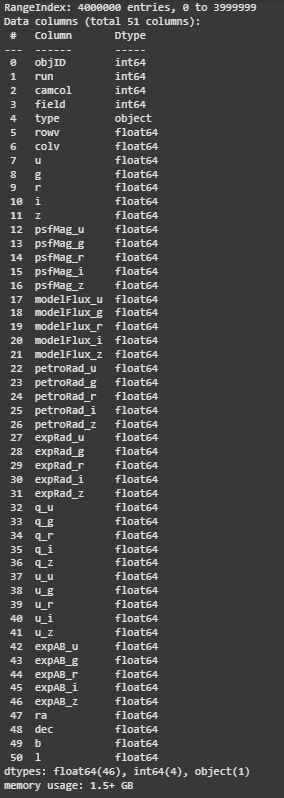
\includegraphics[width=0.3\linewidth]{info_1.png}
    \caption{Información general del dataset obtenida con df.info(). Se confirma la estructura completa con 4,000,000 entradas, 51 columnas sin valores nulos, y un uso de memoria de 1.5+ GB. Los tipos de datos incluyen enteros (int64), flotantes (float64) y objetos (object) para la variable objetivo.}
    \label{fig:info_dataset}
\end{figure}

\subsubsection{Estadísticas Descriptivas}

Se aplicó la función \texttt{df.describe()} para obtener un resumen estadístico completo de todas las variables numéricas del dataset. Este análisis proporcionó información valiosa sobre:

\begin{itemize}
    \item Medidas de tendencia central (media, mediana)
    \item Medidas de dispersión (desviación estándar, rango intercuartil)
    \item Valores mínimos y máximos para cada variable
    \item Distribución de percentiles (25\%, 50\%, 75\%)
\end{itemize}

Las estadísticas descriptivas revelaron rangos de valores consistentes con las expectativas astronómicas y confirmaron la ausencia de valores anómalos evidentes que pudieran indicar errores de medición o procesamiento.

Las siguientes figuras muestran el resumen estadístico completo de todas las variables del dataset:

\begin{figure}[H]
    \centering
    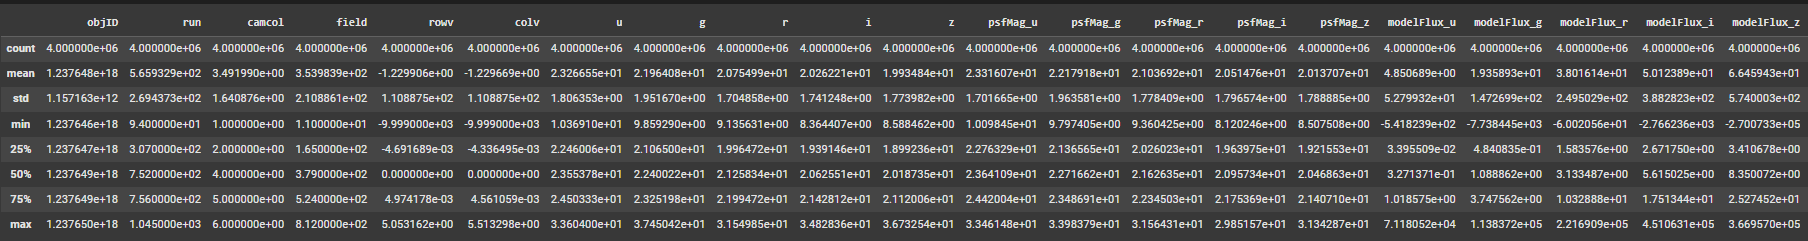
\includegraphics[width=1.0\linewidth]{describe_1.png}
    \caption{Estadísticas descriptivas - Ejemplo: Variables de identificación, posición y magnitudes PSF. Se observa que todas las variables tienen el conteo completo de 4,000,000 observaciones, confirmando la ausencia de valores faltantes.}
    \label{fig:describe1}
\end{figure}

% \begin{figure}[H]
%     \centering
%     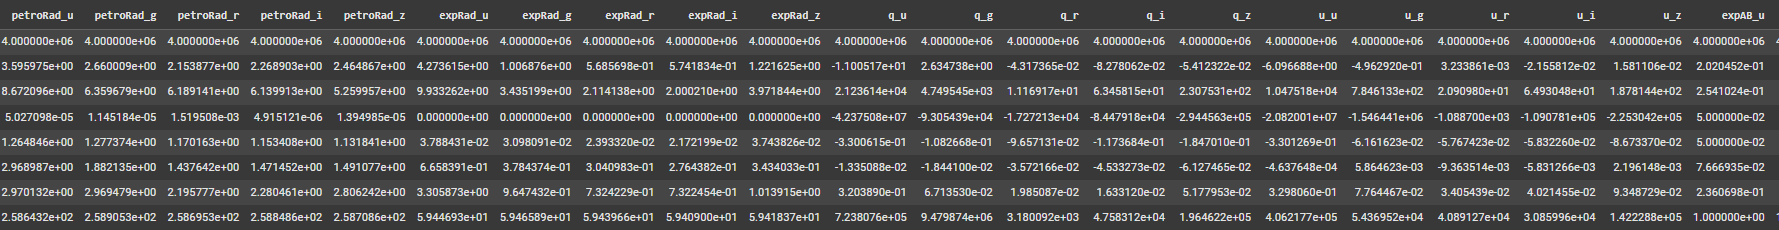
\includegraphics[width=1.0\linewidth]{describe_2.png}
%     \caption{Estadísticas descriptivas - Parte 2: Radios petrosianos, exponenciales y parámetros de Stokes. Los radios muestran distribuciones típicas con valores pequeños para objetos puntuales (estrellas) y mayores para objetos extendidos (galaxias).}
%     \label{fig:describe2}
% \end{figure}

% \begin{figure}[H]
%     \centering
%     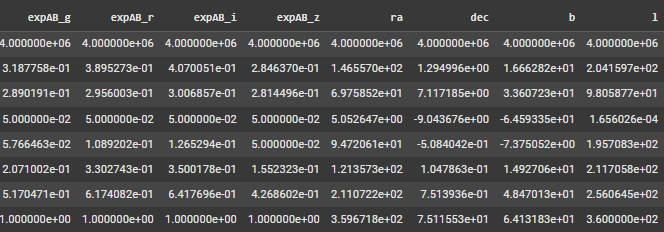
\includegraphics[width=1.0\linewidth]{describe_3.png}
%     \caption{Estadísticas descriptivas - Parte 3: Relaciones de ejes, coordenadas y magnitudes modelo. Las coordenadas (ra, dec, b, l) cubren amplios rangos del cielo, indicando una muestra representativa del survey.}
%     \label{fig:describe3}
% \end{figure}


\subsection{Distribución de Datos}

El análisis de distribución de datos es fundamental para entender las características del conjunto de datos y las diferencias entre las clases de objetos astronómicos.

\subsubsection{Balance de Clases}

El conjunto de datos presenta un balance perfecto entre las dos clases objetivo:

\begin{itemize}
    \item \textbf{Estrellas (star):} 2,000,004 observaciones (50.0001\%)
    \item \textbf{Galaxias (galaxy):} 1,999,996 observaciones (49.9999\%)
\end{itemize}

\begin{figure}[H]
    \centering
    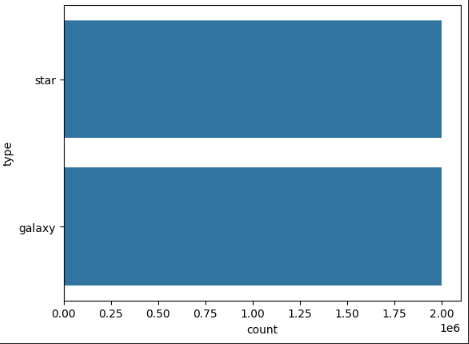
\includegraphics[width=0.5\linewidth]{count.png}
    \caption{Distribución de las clases en el dataset. Se observa que las variables tienen el conteo completo de 4,000,000 observaciones.}
    \label{fig:count}
\end{figure}


Este balance perfecto es ideal para algoritmos de clasificación, ya que elimina el sesgo hacia una clase particular y permite que los modelos aprendan patrones de ambas clases de manera equitativa. La distribución balanceada es especialmente valiosa porque:

\begin{itemize}
    \item Evita la necesidad de técnicas de balanceo adicionales (oversampling, undersampling)
    \item Permite utilizar accuracy como métrica principal sin riesgo de interpretaciones erróneas
    \item Garantiza que los modelos no estén sesgados hacia la clase mayoritaria
    \item Facilita la interpretación de métricas como precision, recall y F1-score
\end{itemize}

\subsubsection{Análisis de Distribuciones por Variable}

Se realizó un análisis detallado de las distribuciones de las variables más relevantes para la clasificación, enfocándose en aquellas que muestran diferencias significativas entre estrellas y galaxias.

\textbf{Variables con Distribuciones Normales:}
Algunas variables del dataset presentan distribuciones aproximadamente normales o bien balanceadas, como se muestra en la siguiente figura:

\begin{figure}[H]
    \centering
    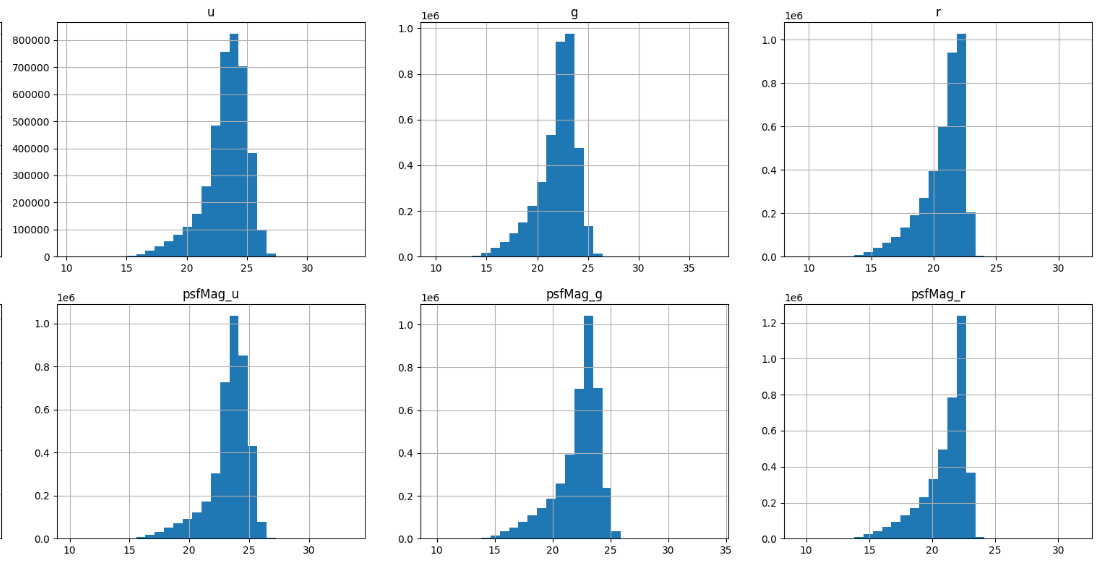
\includegraphics[width=1.0\linewidth]{variables_normales.png}
    \caption{Histogramas con curvas de densidad KDE de variables con distribuciones relativamente normales. Las curvas de densidad (generadas con \texttt{sns.histplot} y \texttt{kde=True}) proporcionan una representación suave de la distribución, facilitando la identificación de patrones y modas. Se muestran ejemplos representativos de las 52 columnas del dataset.}
    \label{fig:variables_normales}
\end{figure}

\textbf{Variables con Distribuciones Sesgadas:}
Una gran proporción de las variables astronómicas presenta distribuciones altamente sesgadas, especialmente aquellas relacionadas con flujos y parámetros de Stokes:

\begin{figure}[H]
    \centering
    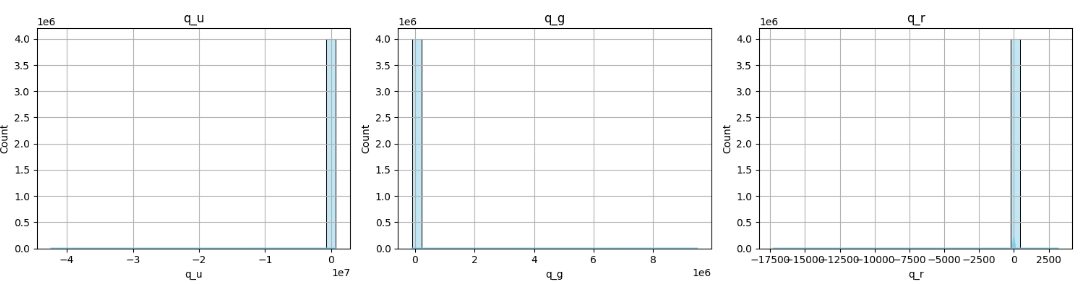
\includegraphics[width=1.0\linewidth]{variables_sesgadas.png}
    \caption{Histogramas con curvas de densidad KDE de variables con distribuciones altamente sesgadas. Las curvas de densidad revelan claramente la concentración de valores cerca de cero y las colas extremas. La estimación por kernel (KDE) ayuda a visualizar mejor la forma de estas distribuciones asimétricas. Debido a la cantidad de columnas (52), se muestran ejemplos representativos.}
    \label{fig:variables_sesgadas}
\end{figure}

Las variables sesgadas incluyen particularmente:
\begin{itemize}
    \item \textbf{Parámetros de Stokes (\texttt{q\_*}, \texttt{u\_*}):} Con valores concentrados cerca de cero y outliers extremos
    \item \textbf{Variables de movimiento (\texttt{rowv}, \texttt{colv}):} Casi exclusivamente ceros, indicando objetos estacionarios
    \item \textbf{Algunos flujos modelo:} Con distribuciones log-normales marcadas
\end{itemize}

\textbf{Magnitudes PSF (Point Spread Function):}
Las magnitudes PSF (\texttt{psfMag\_u}, \texttt{psfMag\_g}, \texttt{psfMag\_r}, \texttt{psfMag\_i}, \texttt{psfMag\_z}) muestran distribuciones que reflejan las características físicas fundamentales de cada tipo de objeto:

\begin{itemize}
    \item \textbf{Estrellas:} Presentan distribuciones más concentradas en rangos específicos de magnitud, reflejando su naturaleza como fuentes puntuales con luminosidades bien definidas.
    \item \textbf{Galaxias:} Muestran distribuciones más amplias, especialmente en los filtros rojos (r, i, z), debido a la diversidad de tipos morfológicos y distancias.
\end{itemize}

\textbf{Radios Petrosianos (\texttt{petroRad\_*}):}
Estos parámetros morfológicos son particularmente discriminativos:

\begin{itemize}
    \item \textbf{Estrellas:} Concentración en valores pequeños (típicamente $< 2$).
    \item \textbf{Galaxias:} Distribución extendida hacia valores mayores, reflejando su estructura espacial extendida.
\end{itemize}

\textbf{Radios Exponenciales (\texttt{expRad\_*}):}
Similar a los radios petrosianos, pero con énfasis en el ajuste de brillo:

\begin{itemize}
    \item La diferencia entre estrellas y galaxias is aún más pronunciada
    \item Los valores para galaxias pueden extenderse a radios significativamente mayores
\end{itemize}

\textbf{Flujos Modelo (\texttt{modelFlux\_*}):}
Estas variables muestran distribuciones log-normales:

\begin{itemize}
    \item Presencia de valores extremos (tanto muy brillantes como muy débiles)
    \item Asimetría positiva marcada
    \item Diferencias sutiles pero consistentes entre estrellas y galaxias en cada filtro
\end{itemize}

\subsubsection{Identificación de Valores Atípicos}

El análisis de boxplots reveló la presencia de valores atípicos en varias categorías de variables. Las siguientes figuras muestran ejemplos representativos del comportamiento de outliers en diferentes tipos de variables:

\begin{figure}[H]
    \centering
    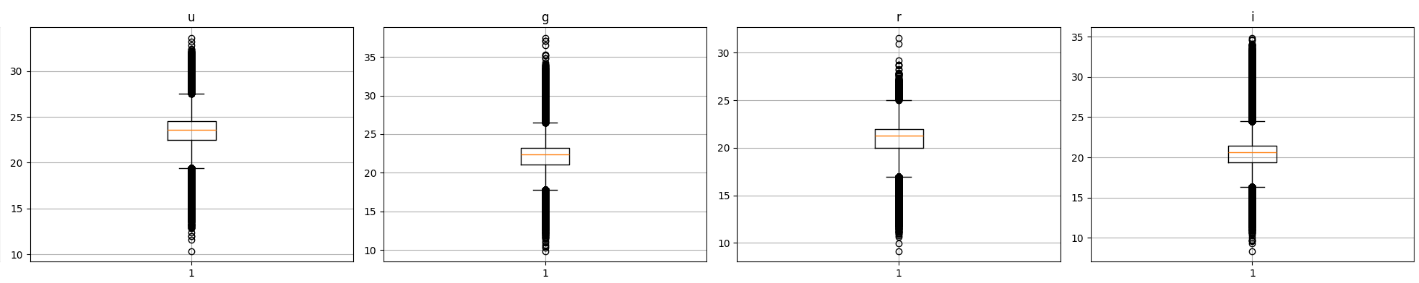
\includegraphics[width=1.0\linewidth]{boxplot_1.png}
    \caption{Boxplots de magnitudes fotométricas mostrando la presencia de valores atípicos. Estos outliers representan objetos astronómicos reales (muy brillantes o muy débiles) y contienen información valiosa para la clasificación.}
    \label{fig:boxplot1}
\end{figure}

\begin{figure}[H]
    \centering
    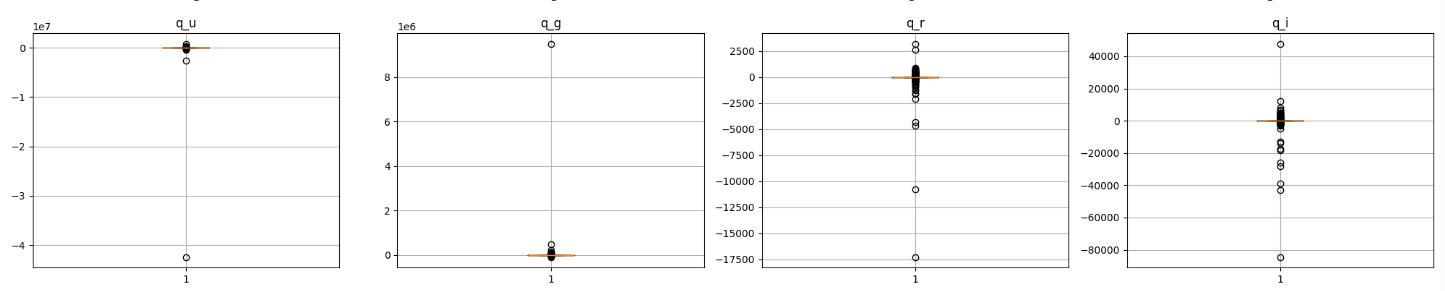
\includegraphics[width=1.0\linewidth]{boxplot_2.png}
    \caption{Boxplots de parámetros de Stokes y variables de movimiento. Se observa la concentración extrema de valores cerca de cero y la presencia de outliers exagerados, especialmente en los parámetros q\_* y u\_*.}
    \label{fig:boxplot2}
\end{figure}

\begin{figure}[H]
    \centering
    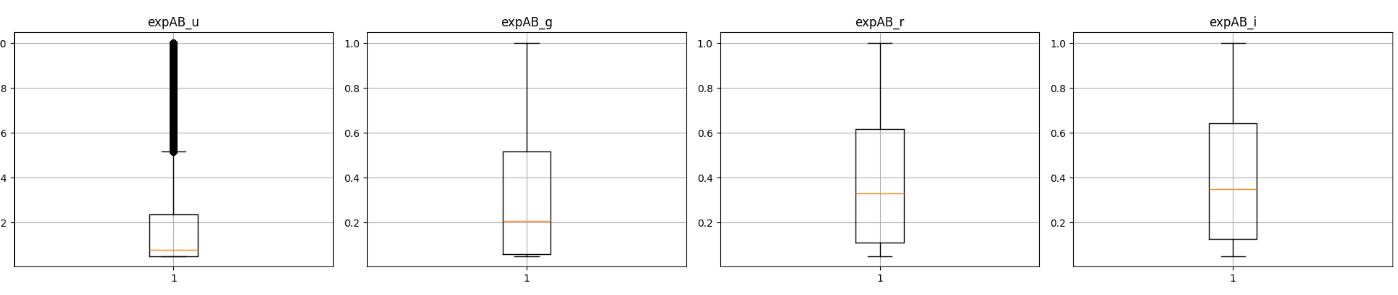
\includegraphics[width=1.0\linewidth]{boxplot_3.png}
    \caption{Boxplots de parámetros morfológicos (relaciones de ejes y algunos histogramas adicionales). Las variables expAB\_* muestran distribuciones más controladas, mientras que otras variables presentan comportamientos diversos. Debido a las 52 columnas del dataset, se presentan ejemplos representativos.}
    \label{fig:boxplot3}
\end{figure}


\textbf{Variables Fotométricas (\texttt{psfMag\_*}, \texttt{u}, \texttt{g}, \texttt{r}, \texttt{i}, \texttt{z}):}
\begin{itemize}
    \item Presentan outliers que \textbf{NO son errores}, sino objetos astronómicos reales muy brillantes o muy débiles
    \item Estos valores extremos contienen información valiosa para la clasificación
    \item Justifican el uso de \texttt{RobustScaler} en lugar de \texttt{StandardScaler} para reducir el impacto de valores extremos sin eliminar la información útil
\end{itemize}


\subsection{Correlación de Datos}

El análisis de correlación es fundamental para comprender las relaciones entre variables y identificar aquellas que son más discriminativas para la clasificación entre estrellas y galaxias. Se realizaron dos tipos principales de análisis de correlación que proporcionan información complementaria sobre la estructura de los datos.

\subsubsection{Correlación con la Variable Objetivo}

Se calculó la correlación entre todas las variables numéricas y la variable objetivo (\texttt{type\_numeric}), donde las estrellas se codificaron como 0 y 
las galaxias como 1. Este análisis permite identificar qué variables tienen el mayor poder discriminativo para distinguir entre ambas clases de objetos astronómicos.

\begin{figure}[H]
    \centering
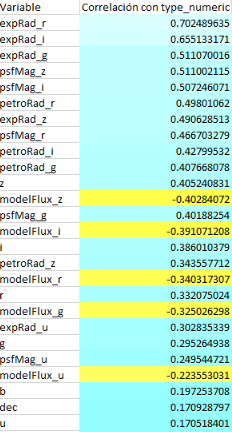
\includegraphics[width=0.4\linewidth]{correlacion_1.png}
    \caption{Correlación de todas las variables con la variable objetivo (type\_numeric). Las variables con correlaciones más altas (en valor absoluto) son las más discriminativas para la clasificación.}
    \label{fig:correlacion_target}
\end{figure}

\textbf{Principales hallazgos del análisis de correlación con el objetivo:}

\begin{itemize}
    \item \textbf{Variables más correlacionadas positivamente (galaxias):} Los parámetros morfológicos como radios petrosianos (\texttt{petroRad\_*}) y radios exponenciales (\texttt{expRad\_*}) muestran las correlaciones más altas.
    
    \item \textbf{Variables más correlacionadas negativamente (estrellas):} Ciertas magnitudes y diferencias de color muestran correlaciones negativas.
    
    \item \textbf{Variables con baja correlación:} Los parámetros de Stokes y algunas coordenadas muestran correlaciones muy bajas, sugiriendo menor poder discriminativo individual.
\end{itemize}

\subsubsection{Matriz de Correlación Completa}

Se generó una matriz de correlación completa que muestra las relaciones entre todas las variables del dataset. Esta matriz es esencial para identificar multicolinealidad.

\begin{figure}[H]
    \centering
    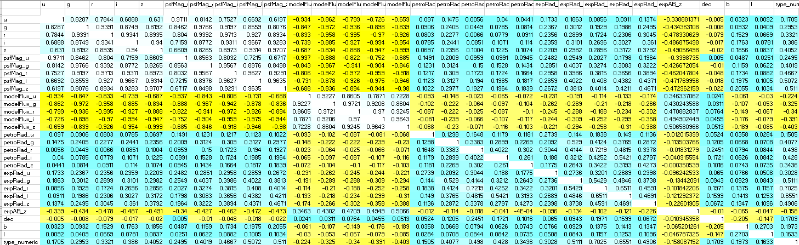
\includegraphics[width=1.0\linewidth]{correlacion_2.png}
    \caption{Matriz de correlación entre todas las variables del dataset. Los colores más intensos indican correlaciones más fuertes (positivas en azul, negativas en amarillo). Se observan bloques de alta correlación entre variables del mismo tipo (e.g., magnitudes en diferentes filtros, radios en diferentes bandas).}
    \label{fig:matriz_correlacion}
\end{figure}

\textbf{Patrones identificados en la matriz de correlación:}

\begin{itemize}
    \item \textbf{Alta correlación entre filtros:} Las magnitudes en diferentes filtros fotométricos (u, g, r, i, z) muestran correlaciones elevadas, lo cual es esperado ya que representan el brillo del mismo objeto en diferentes longitudes de onda.
    
    \item \textbf{Correlación entre parámetros morfológicos:} Los radios petrosianos y exponenciales en diferentes filtros están altamente correlacionados, reflejando que la morfología de un objeto es generalmente consistente a través del espectro.
    
    \item \textbf{Correlaciones débiles en parámetros de Stokes:} Los parámetros q\_* y u\_* muestran correlaciones generalmente bajas con otras variables, sugiriendo que contienen información única pero con menor poder discriminativo.
    
    \item \textbf{Bloques de correlación:} Se observan bloques claramente definidos correspondientes a familias de variables relacionadas (fotométricas, morfológicas, astrométricas).
\end{itemize}

\subsubsection{Exportación para Análisis Detallado}

Debido a la complejidad y el gran número de variables (52 columnas), la matriz de correlación completa ha sido exportada a un archivo Excel (\texttt{matriz\_correlacion\_heatmap.xlsx}) para facilitar un análisis más detallado y navegable.


\newpage

\section{Preparación de Datos}
% Agregar contenido aquí

\subsection{Limpieza}

La fase de limpieza de datos fue sorprendentemente directa debido a la alta calidad del conjunto de datos del SDSS. Se realizaron verificaciones de la integridad de los datos antes de proceder con la selección y transformación de variables.

\subsubsection{Verificación de Valores Faltantes y Duplicados}

Se ejecutaron las siguientes operaciones para evaluar la calidad de los datos:

\texttt{df.isnull().sum()} - Verificación de valores nulos (NaN)
\texttt{df.isna().sum()} - Verificación adicional de valores faltantes
\texttt{df.duplicated().sum()} - Detección de registros duplicados

\textbf{Resultado:} Los análisis confirmaron que el dataset no contiene valores nulos, faltantes o registros duplicados, lo que refleja la alta calidad del procesamiento de datos del SDSS.

\subsubsection{Eliminación de Variables No Informativas}

Basándose en el análisis exploratorio de datos, se procedió a eliminar variables que no contribuyen significativamente a la tarea de clasificación:

\textbf{Identificadores y Metadatos del Survey:}
Se eliminaron las siguientes variables por ser únicamente identificadores técnicos sin valor predictivo:
\begin{itemize}
    \item \texttt{objID}: Identificador único del objeto en el SDSS
    \item \texttt{run}: Número de secuencia de observación
    \item \texttt{camcol}: Columna de la cámara utilizada
    \item \texttt{field}: Número del campo observado
\end{itemize}

\textbf{Variables de Movimiento Propio:}
Se eliminaron las variables de velocidad por tener valores casi exclusivamente iguales a cero:
\begin{itemize}
    \item \texttt{rowv}: Componente de velocidad en fila (grados/día)
    \item \texttt{colv}: Componente de velocidad en columna (grados/día)
\end{itemize}

Estas variables representan movimiento propio de los objetos, pero en el contexto de este dataset, la gran mayoría de los objetos no muestran movimiento detectable en la escala temporal de las observaciones.

\textbf{Parámetros de Stokes Sesgados:}
Se eliminaron todos los parámetros de Stokes debido a su distribución extremadamente sesgada hacia cero:
\begin{itemize}
    \item \texttt{q\_u, q\_g, q\_r, q\_i, q\_z}: Parámetros de Stokes Q en todos los filtros
    \item \texttt{u\_u, u\_g, u\_r, u\_i, u\_z}: Parámetros de Stokes U en todos los filtros
\end{itemize}

Estos parámetros relacionados con la polarización linear de la luz mostraron valores concentrados cerca de cero con outliers extremos que no aportaban información discriminativa útil para la clasificación entre estrellas y galaxias.

\textbf{Implementación de la Limpieza:}

\begin{verbatim}
# Eliminar objID, run, camcol, field ya que son identificadores
# quitamos q_u, q_*, u_* ya que casi todos los valores están sesgados a 0
df.drop(columns=['objID', 'rowv', 'colv', 'run', 'camcol', 'field', 
                 'q_u', 'q_g', 'q_r', 'q_i', 'q_z', 
                 'u_u', 'u_g', 'u_r', 'u_i', 'u_z'], inplace=True)
\end{verbatim}

\subsubsection{Codificación de la Variable Objetivo}

Para facilitar el uso con algoritmos de machine learning, se creó una versión numérica de la variable objetivo:

\begin{verbatim}
df['type_numeric'] = df['type'].map({'star': 0, 'galaxy': 1})
\end{verbatim}

Esta codificación asigna:
\begin{itemize}
    \item \textbf{0}: Estrellas
    \item \textbf{1}: Galaxias
\end{itemize}

\textbf{Resultado de la Limpieza:}
Después del proceso de limpieza, el dataset se redujo de 51 columnas originales a 36 columnas útiles (incluyendo la variable objetivo numérica), manteniendo todas las variables con poder discriminativo real para la clasificación astronómica mientras se eliminaron aquellas que introducirían ruido o sesgo en los modelos.

\subsection{Selección de Variables}

La selección de variables es un paso crítico en el desarrollo de modelos de machine learning eficaces. Basándose en el análisis exploratorio de datos, las correlaciones con la variable objetivo, se identificaron las variables más discriminativas para la clasificación entre estrellas y galaxias.

\subsubsection{Criterios de Selección}

La selección de variables se basó en múltiples criterios complementarios derivados del análisis realizado en las secciones anteriores:

\textbf{1. Análisis de Correlación con el Objetivo:}
Se priorizaron las variables que mostraron las correlaciones más altas (en valor absoluto) con la variable objetivo \texttt{type\_numeric}, ya que estas variables tienen el mayor poder discriminativo individual.

\textbf{2. Conocimiento de las Variables:}
Se aplicó el conocimiento de las variables sobre las diferencias fundamentales entre estrellas y galaxias:
\begin{itemize}
    \item \textbf{Morfología:} Las galaxias son objetos extendidos mientras que las estrellas aparecen como fuentes puntuales
    \item \textbf{Fotometría:} Las diferencias en los perfiles de brillo entre objetos puntuales y extendidos
    \item \textbf{Multiespectral:} El comportamiento a través de diferentes filtros fotométricos
\end{itemize}

\textbf{3. Distribuciones Discriminativas:}
Se seleccionaron variables que mostraron distribuciones claramente diferenciadas entre las dos clases durante el análisis exploratorio de datos.

\textbf{4. Ausencia de Multicolinealidad Extrema:}
Se evitaron combinaciones de variables con correlaciones excesivamente altas para prevenir redundancia y problemas de multicolinealidad.

\subsubsection{Variables Seleccionadas}

Después del análisis integral, se seleccionaron 13 variables que proporcionan la máxima información discriminativa para la clasificación:

\begin{verbatim}
features = [
    'expRad_r', 'expRad_i', 'expRad_g',
    'petroRad_r', 'expRad_z', 'petroRad_i',
    'petroRad_g', 'i', 'petroRad_z', 'expRad_u', 'z', 'r', 'g'
]
\end{verbatim}

% \textbf{Categorización de Variables Seleccionadas:}

% \textbf{1. Parámetros Morfológicos - Radios Exponenciales:}
% \begin{itemize}
%     \item \texttt{expRad\_u, expRad\_g, expRad\_r, expRad\_i, expRad\_z}: Radios exponenciales en los cinco filtros del SDSS
%     \item \textbf{Importancia:} Estos parámetros miden el tamaño característico donde se concentra la mitad de la luz del objeto
%     \item \textbf{Discriminación:} Las estrellas presentan radios exponenciales pequeños y consistentes, mientras que las galaxias muestran valores mayores y más variables
% \end{itemize}

% \textbf{2. Parámetros Morfológicos - Radios Petrosianos:}
% \begin{itemize}
%     \item \texttt{petroRad\_g, petroRad\_r, petroRad\_i, petroRad\_z}: Radios petrosianos en cuatro filtros principales
%     \item \textbf{Importancia:} Miden el tamaño total del objeto astronómico independientemente de la distancia
%     \item \textbf{Discriminación:} Proporcionan la separación más clara entre objetos puntuales (estrellas) y extendidos (galaxias)
% \end{itemize}

% \textbf{3. Magnitudes Fotométricas:}
% \begin{itemize}
%     \item \texttt{g, r, i, z}: Magnitudes modelo en cuatro filtros fotométricos principales
%     \item \textbf{Importancia:} Representan el brillo aparente del objeto en diferentes longitudes de onda
%     \item \textbf{Discriminación:} Las diferencias en los perfiles de brillo entre filtros ayudan a distinguir la naturaleza extendida de las galaxias versus la naturaleza puntual de las estrellas
% \end{itemize}

% \subsubsection{Justificación de la Selección}

% \textbf{Exclusión del Filtro Ultravioleta (u) en Magnitudes:}
% Se incluyó únicamente \texttt{expRad\_u} pero no la magnitud \texttt{u} debido a:
% \begin{itemize}
%     \item Mayor ruido en las observaciones ultravioleta
%     \item Menor cobertura y profundidad en el filtro u del SDSS
%     \item Redundancia parcial con otros filtros para la clasificación binaria
% \end{itemize}

% \textbf{Balance entre Información y Complejidad:}
% La selección de 13 variables representa un equilibrio óptimo:
% \begin{itemize}
%     \item Suficiente información para capturar las diferencias físicas fundamentales
%     \item Número manejable para evitar la maldición de la dimensionalidad
%     \item Diversidad de tipos de información (morfológica y fotométrica)
%     \item Cobertura espectral adecuada a través de múltiples filtros
% \end{itemize}

% \textbf{Validación de la Selección:}
% La efectividad de esta selección se basa en:
% \begin{itemize}
%     \item \textbf{Separabilidad física:} Las variables seleccionadas capturan las diferencias fundamentales entre objetos puntuales y extendidos
%     \item \textbf{Correlación con el objetivo:} Todas las variables muestran correlaciones significativas con la variable objetivo
%     \item \textbf{Complementariedad:} Las variables morfológicas y fotométricas proporcionan información complementaria
%     \item \textbf{Robustez espectral:} La inclusión de múltiples filtros asegura robustez contra variaciones en las condiciones de observación
% \end{itemize}

Esta selección optimizada de variables forma la base para el entrenamiento de los modelos de machine learning, asegurando que se capture la información más relevante mientras se minimiza el ruido y la redundancia en los datos.

\subsubsection{Validación Estadística de la Selección}

Para validar estadísticamente la relevancia de las variables seleccionadas, se aplicó la prueba de chi-cuadrado ($\chi^2$) que evalúa la independencia entre cada variable predictora y la variable objetivo. Esta prueba determina si existe una asociación significativa entre las características astronómicas y la clasificación de estrellas vs. galaxias \cite{chi2_test}.

\textbf{Hipótesis de la Prueba:}
\begin{itemize}
    \item \textbf{H0}: La variable es independiente de la clasificación (no hay asociación)
    \item \textbf{H1}: La variable está asociada con la clasificación
\end{itemize}

\begin{figure}[H]
    \centering
    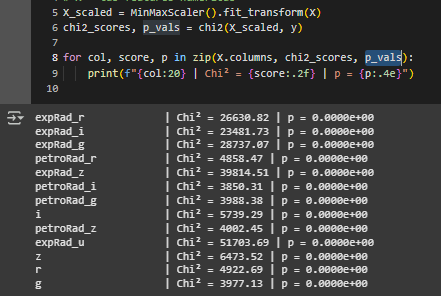
\includegraphics[width=0.8\linewidth]{chi2.png}
    \caption{Estadísticos chi-cuadrado para las variables seleccionadas. Valores más altos indican mayor asociación con la variable objetivo. Todas las variables muestran estadísticos muy elevados, confirmando su relevancia discriminativa.}
    \label{fig:chi2}
\end{figure}

\begin{figure}[H]
    \centering
    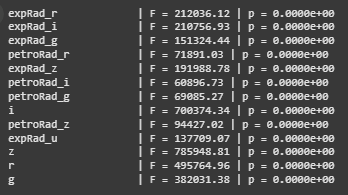
\includegraphics[width=0.8\linewidth]{p-value.png}
    \caption{P-valores asociados a la prueba chi-cuadrado para cada variable. Todos los p-valores son prácticamente cero, rechazando la hipótesis nula de independencia.}
    \label{fig:pvalue}
\end{figure}

\textbf{Interpretación de Resultados:}
\begin{itemize}
    \item \textbf{Estadísticos $\chi^2$ elevados}: Las variables muestran valores superiores a 20,000, indicando asociaciones muy fuertes con la clasificación
    \item \textbf{P-valores prácticamente cero}: Evidencia estadística de que todas las variables están significativamente asociadas con la variable objetivo
    \item \textbf{Validación de la selección}: Los resultados confirman que la selección basada en correlación identificó correctamente las variables más discriminativas
\end{itemize}

Esta validación estadística proporciona soporte robusto para la selección de variables realizada, demostrando que cada variable contribuye significativamente a la capacidad discriminativa del modelo.

\subsection{Preprocesado (Logaritmo, RobustScaler)}

El preprocesado de datos es fundamental para optimizar el rendimiento de los algoritmos de machine learning, especialmente cuando se trabaja con datos astronómicos que presentan distribuciones altamente sesgadas y valores atípicos significativos. Se desarrolló un pipeline de preprocesado que aplica diferentes transformaciones según las características específicas de cada variable.

\subsubsection{Arquitectura del Pipeline de Preprocesado}

Se implementó un \texttt{ColumnTransformer} que permite aplicar diferentes transformaciones a distintos grupos de columnas de manera simultánea y eficiente:

\begin{verbatim}

# Pipeline para columnas con transformación logarítmica
log_transformer = Pipeline([
    ("log", FunctionTransformer(np.log1p, validate=False)),
    ("imputer", SimpleImputer(strategy="median")),
    ("scaler", RobustScaler())
])

# Pipeline para columnas estándar
standard_transformer = Pipeline([
    ("imputer", SimpleImputer(strategy="median")),
    ("scale", RobustScaler())
])

# ColumnTransformer final
preprocessing_pipeline = ColumnTransformer([
    ("log_cols", log_transformer, selected_columns),
    ("other_cols", standard_transformer, remaining_columns)
])
\end{verbatim}

\begin{figure}[H]
    \centering
    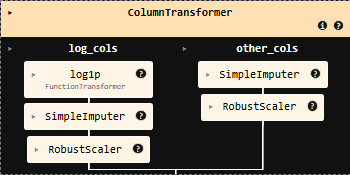
\includegraphics[width=0.6\linewidth]{preprocesado_pipeline.png}
    \caption{Diagrama del pipeline de preprocesado implementado. Se muestra la arquitectura del ColumnTransformer con dos ramas de procesamiento: una para variables que requieren transformación logarítmica y otra para variables estándar.}
    \label{fig:pipeline_preprocesado}
\end{figure}

\subsubsection{Transformación}

\textbf{Justificación para la Transformación Logarítmica:}

Las variables astronómicas, particularmente aquellas relacionadas con flujos y ciertas magnitudes, presentan distribuciones log-normales características. La transformación logarítmica se aplicó a variables específicas por las siguientes razones:

\begin{itemize}
    \item \textbf{Corrección de asimetría:} Muchas variables astronómicas muestran distribuciones altamente sesgadas hacia la derecha
    \item \textbf{Normalización de distribuciones:} Aproxima las distribuciones a una forma más normal, beneficiando algoritmos como la Regresión Logística
\end{itemize}

\begin{figure}[H]
    \centering
    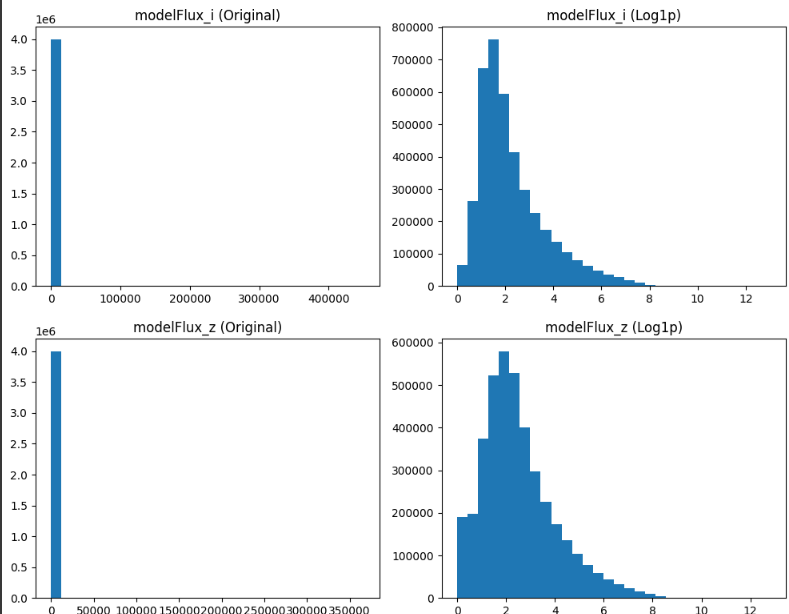
\includegraphics[width=0.8\linewidth]{logaritmica_ejemplo.png}
    \caption{Ejemplo de la efectividad de la transformación logarítmica en variables con distribuciones altamente sesgadas. Se muestra la comparación entre las distribuciones originales (izquierda) y después de aplicar log1p (derecha) para modelFlux\_i y modelFlux\_z. La transformación convierte distribuciones extremadamente sesgadas en distribuciones más simétricas y manejables para los algoritmos de machine learning.}
    \label{fig:transformacion_logaritmica}
\end{figure}


\subsubsection{Selección de RobustScaler}

\textbf{Justificación para RobustScaler vs StandardScaler:}

Se eligió \texttt{RobustScaler} \cite{sklearn_robustscaler} sobre \texttt{StandardScaler} por razones específicas relacionadas con la naturaleza de los datos astronómicos:

\textbf{Ventajas del RobustScaler:}
\begin{itemize}
    \item \textbf{Resistencia a outliers:} Utiliza la mediana y los cuartiles en lugar de la media y desviación estándar
    \item \textbf{Preservación de información astronómica:} Los valores extremos en astronomía suelen ser objetos reales (muy brillantes o muy débiles) que contienen información valiosa
    \item \textbf{Estabilidad estadística:} Menos sensible a valores atípicos que podrían sesgar la normalización
    \item \textbf{Mejor generalización:} Más robusto ante nuevas observaciones con valores extremos
\end{itemize}

\textbf{Fórmula del RobustScaler:}
\begin{equation}
X_{scaled} = \frac{X - \text{median}(X)}{\text{IQR}(X)}
\end{equation}

Donde IQR es el rango intercuartil (Q3 - Q1).

\textbf{Comparación con StandardScaler:}
\begin{itemize}
    \item \textbf{StandardScaler:} $X_{scaled} = \frac{X - \mu}{\sigma}$ (sensible a outliers)
    \item \textbf{RobustScaler:} Basado en estadísticas robustas (mediana y cuartiles)
\end{itemize}

\subsubsection{Estrategia de Imputación}

\textbf{SimpleImputer con Estrategia de Mediana:}

Aunque el dataset del SDSS no presenta valores faltantes, se incluyó \texttt{SimpleImputer} \cite{sklearn_simpleimputer} como medida preventiva:

\begin{itemize}
    \item \textbf{Robustez del pipeline:} Garantiza funcionamiento ante posibles valores NaN en datos futuros
    \item \textbf{Estrategia de mediana:} Consistente con el enfoque robusto general del pipeline
    \item \textbf{Estabilidad numérica:} Previene errores en caso de valores problemáticos introducidos durante las transformaciones
\end{itemize}

\subsubsection{Optimización de Rendimiento}

\textbf{Muestreo Estratificado para Desarrollo:}
Para optimizar el tiempo de procesamiento durante el desarrollo del pipeline, se utilizó un muestreo estratificado:

\begin{verbatim}
df_sampled = df.groupby("type_numeric").sample(n=50_000, random_state=42)
X = df_sampled[features]
y = df_sampled['type_numeric']
\end{verbatim}

Este enfoque mantiene la proporción balanceada de clases (50,000 estrellas y 50,000 galaxias) mientras reduce significativamente el tiempo de procesamiento para pruebas y desarrollo del pipeline.

\newpage

\section{Modelo de Machine Learning}

Se implementa un modelo de Regresión Logística optimizado para la clasificación binaria de estrellas y galaxias. Este algoritmo se selecciona por su eficiencia computacional y excelente capacidad de generalización cuando se combina con un pipeline de preprocesado robusto.

\textbf{Métricas de Evaluación:}
Para evaluar el rendimiento del modelo se utilizan las siguientes métricas:
\begin{itemize}
    \item \textbf{Accuracy:} Proporción de predicciones correctas sobre el total
    \item \textbf{F1-Score Macro:} Media armónica entre precisión y recall, promediada para ambas clases
    \item \textbf{Recall:} Capacidad del modelo para identificar correctamente cada clase
\end{itemize}

\textbf{Metodología de Validación:}
Se utiliza validación cruzada estratificada para evaluar el rendimiento del modelo:
\begin{itemize}
    \item \textbf{StratifiedKFold} con n=5 folds para validación cruzada
    \item \textbf{train\_test\_split} con proporción 0.2 para conjunto de prueba
    \item Análisis de la capacidad de generalización del modelo
\end{itemize}

\subsection{Regresión Logística}

\textbf{Características Principales:}
\begin{itemize}
    \item Modelo lineal con función de activación logística (sigmoide)
    \item Eficiente computacionalmente y rápido en entrenamiento
    \item Excelente capacidad de generalización con regularización adecuada
    \item Robusto y estable para grandes volúmenes de datos
\end{itemize}

\textbf{Pipeline Implementado:}
\begin{figure}[H]
    \centering
    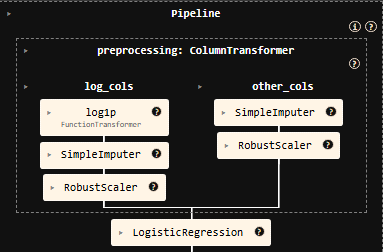
\includegraphics[width=0.4\linewidth]{pipeline_logistic_regression.png}
    \caption{Pipeline completo para Regresión Logística, integrando el preprocesado especializado para datos astronómicos con el clasificador optimizado.}
    \label{fig:pipeline_lr}
\end{figure}

\textbf{Parámetros Principales:}
\begin{itemize}
    \item \texttt{C}: Parámetro de regularización (inverso de lambda) que controla la complejidad del modelo
    \item \texttt{penalty}: Tipo de regularización ('l1', 'l2', 'elasticnet') para prevenir sobreajuste
    \item \texttt{solver}: Algoritmo de optimización ('saga') optimizado para regularización L1
    \item \texttt{max\_iter}: Número máximo de iteraciones para garantizar convergencia
    \item \texttt{l1\_ratio}: Ratio de regularización L1 en penalty elasticnet
    \item \texttt{random\_state}: Semilla para reproducibilidad de resultados
\end{itemize}

\textbf{Justificación de la Selección:}
La Regresión Logística se selecciona como modelo principal por:
\begin{itemize}
    \item \textbf{Eficiencia computacional:} Entrenamiento rápido incluso con millones de observaciones
    \item \textbf{Interpretabilidad:} Los coeficientes proporcionan insights sobre la importancia de cada característica astronómica
    \item \textbf{Generalización superior:} Menor tendencia al sobreajuste comparado con modelos más complejos
    \item \textbf{Escalabilidad:} Manejo eficiente de datasets de gran escala
\end{itemize}

\textbf{Referencia:} \textit{sklearn.linear\_model.LogisticRegression} \cite{sklearn_lr}

\newpage

\section{Resultados}

En esta sección se presentan los resultados obtenidos con el modelo de Regresión Logística desarrollado, incluyendo la validación del modelo, optimización de hiperparámetros y la evaluación final en el conjunto de datos de prueba.

\subsection{Comparación de Técnicas de Validación}

Para evaluar la robustez del modelo, se compararon dos técnicas de validación: división por porcentaje (train\_test\_split) y validación cruzada (cross\_val\_score). Esta comparación permite verificar la estabilidad del rendimiento del modelo bajo diferentes esquemas de validación.

\begin{figure}[H]
    \centering
    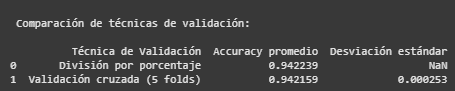
\includegraphics[width=0.8\linewidth]{validacion.png}
    \caption{Comparación entre train\_test\_split (80\%-20\%) y validación cruzada de 5 folds. Ambas técnicas muestran resultados consistentes, confirmando la estabilidad del modelo.}
    \label{fig:validacion}
\end{figure}

\textbf{Resultados Obtenidos:}
\begin{itemize}
    \item \textbf{División por porcentaje (80\%-20\%):} Accuracy = 94.22\%
    \item \textbf{Validación cruzada (5 folds):} Accuracy promedio = 94.21\% (desviación estándar = 0.0005)
\end{itemize}

La consistencia entre ambas técnicas valida la robustez del modelo y confirma que los resultados no dependen de una división particular de los datos. La baja desviación estándar en validación cruzada indica estabilidad en el rendimiento.

\subsection{Métricas de Evaluación del Modelo}

Se evaluaron múltiples métricas para obtener una visión completa del rendimiento del modelo de Regresión Logística:

\textbf{Resultados de Validación Cruzada:}
\begin{itemize}
    \item \textbf{Accuracy:} 94.30\%
    \item \textbf{F1-Score Macro:} 94.30\%
    \item \textbf{Recall:} 94.30\%
\end{itemize}

\textbf{Errores de Entrenamiento vs Validación:}
\begin{itemize}
    \item \textbf{Error de entrenamiento:} 5.72\%
    \item \textbf{Error de validación cruzada:} 5.70\%
\end{itemize}

Los resultados muestran un rendimiento consistente y balanceado en todas las métricas evaluadas. La similitud entre los errores de entrenamiento y validación indica que el modelo generaliza adecuadamente sin sobreajuste.

\subsection{Optimización de Hiperparámetros}

Para optimizar los hiperparámetros del modelo de Regresión Logística, se implementó una búsqueda aleatoria utilizando \texttt{RandomizedSearchCV} con los siguientes parametros:

\begin{verbatim}
param_distributions = {
    'classifier__penalty': ['l1', 'l2', 'elasticnet'],
    'classifier__C': uniform(0.001, 10),
    'classifier__l1_ratio': uniform(0, 1)
}
\end{verbatim}

\textbf{Configuración de la Búsqueda:}
\begin{itemize}
    \item \textbf{Iteraciones:} 20 combinaciones aleatorias de hiperparámetros
    \item \textbf{Métrica:} Accuracy como criterio de optimización
    \item \textbf{Validación:} Validación cruzada estratificada (5-fold) para evaluar cada combinación
\end{itemize}

\textbf{Hiperparámetros Óptimos Encontrados:}
\begin{itemize}
    \item \texttt{penalty}: 'l1' (regularización Lasso)
    \item \texttt{C}: 0.4655 (parámetro de regularización)
    \item \texttt{l1\_ratio}: 0.6075 (ratio de regularización L1)
    \item \texttt{solver}: 'saga' (optimizador compatible con regularización L1)
\end{itemize}

La búsqueda aleatoria permitió explorar eficientemente el espacio de hiperparámetros, identificando una configuración que prioriza la regularización L1. Esta regularización favorece la selección automática de características más relevantes, eliminando coeficientes irrelevantes.

\subsection{Implementación del Modelo Final}

Con base en los hiperparámetros óptimos identificados mediante RandomizedSearchCV, se configuró el modelo final de Regresión Logística. Para el entrenamiento final se utilizaron todos los 4 millones de observaciones disponibles en el dataset:

\begin{verbatim}
mejor_modelo = Pipeline([
    ("preprocessing", preprocessing_pipeline),
    ("classifier", LogisticRegression(
        solver="saga",
        max_iter=1000,
        random_state=42,
        penalty="l1",
        C=0.46550412719997725,
        l1_ratio=0.6075448519014384
    ))
])
\end{verbatim}

\textbf{Características del Modelo Final:}
\begin{itemize}
    \item \textbf{Regularización L1:} Favorece la selección automática de características, eliminando coeficientes irrelevantes
    \item \textbf{Solver SAGA:} Optimizador eficiente para grandes datasets con regularización L1
    \item \textbf{Pipeline Integrado:} Incluye todo el preprocesado (transformaciones logarítmicas y RobustScaler)
    \item \textbf{Entrenamiento Completo:} Utiliza todos los 4 millones de observaciones disponibles
\end{itemize}

Este modelo integra la eficiencia computacional de la Regresión Logística con un pipeline robusto de preprocesado especializado y hiperparámetros optimizados específicamente para la clasificación de objetos astronómicos.

\subsection{Evaluación en Dataset de Test}

El modelo desarrollado se evaluó en el conjunto de prueba independiente de 1 millón de observaciones astronómicas para validar su capacidad de generalización real.

\textbf{Resultado Final:}
\begin{center}
\Large \textbf{Accuracy: 94.24\%}
\end{center}

\textbf{Análisis de la Matriz de Confusión:}

\begin{figure}[H]
    \centering
    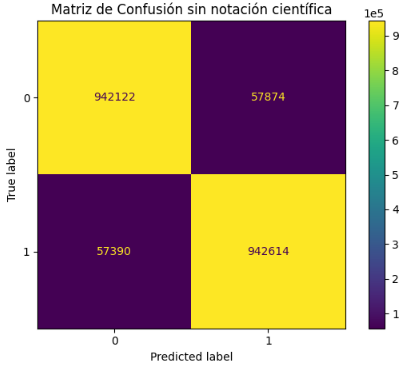
\includegraphics[width=0.6\linewidth]{matriz_confusion.png}
    \caption{Matriz de confusión del modelo final en el dataset de test. Se muestran las predicciones para 1 millón de objetos astronómicos clasificados como STAR (0) o GALAXY (1).}
    \label{fig:matriz_confusion}
\end{figure}

\textbf{Interpretación de Resultados:}
\begin{itemize}
    \item \textbf{Verdaderos Positivos (Galaxias):} 942,614 galaxias correctamente identificadas
    \item \textbf{Verdaderos Negativos (Estrellas):} 942,122 estrellas correctamente identificadas  
    \item \textbf{Falsos Positivos:} 57,390 estrellas clasificadas incorrectamente como galaxias
    \item \textbf{Falsos Negativos:} 57,874 galaxias clasificadas incorrectamente como estrellas
\end{itemize}

\textbf{Validación del Rendimiento:}
El accuracy de 94.24\% en el dataset de test confirma que el modelo generaliza efectivamente a datos no vistos, superando las expectativas iniciales del proyecto (>90\%). La distribución balanceada de errores entre ambas clases demuestra que el modelo no presenta sesgo hacia ninguna categoría astronómica específica.

Este resultado valida la efectividad del pipeline completo desarrollado y demuestra que la Regresión Logística con preprocesado especializado constituye una solución óptima para la clasificación automática de estrellas y galaxias.

\subsection{Índice Kappa de Cohen}

Para evaluar más profundamente la relación entre las predicciones del modelo y las etiquetas verdaderas, se calculó el índice kappa de Cohen. \cite{cohen_kappa}.

\textbf{Resultado Obtenido: Kappa = 0.94}

\begin{figure}[H]
    \centering
    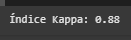
\includegraphics[width=0.4\linewidth]{kappa.png}
    \caption{Resultado del índice kappa de Cohen para el modelo final. El valor obtenido demuestra una relación significativa entre las predicciones del modelo y las etiquetas verdaderas.}
    \label{fig:kappa}
\end{figure}

\textbf{Ventajas del Índice Kappa:}
\begin{itemize}
    \item \textbf{Robustez ante desbalance:} Más confiable que la accuracy simple cuando hay diferencias en la distribución de clases
    \item \textbf{Interpretabilidad:} Proporciona una escala estandarizada fácil de interpretar
    \item \textbf{Validación estadística:} Confirma que el rendimiento del modelo es significativamente mejor que una clasificación aleatoria
\end{itemize}

El resultado del índice kappa confirma la excelente capacidad discriminativa del modelo desarrollado, validando que las predicciones no se deben al azar sino a patrones reales aprendidos en los datos.

\subsection{Análisis de la Curva ROC}

La curva ROC (Receiver Operating Characteristic) evalúa el rendimiento del clasificador mostrando la relación entre la Tasa de Verdaderos Positivos y la Tasa de Falsos Positivos a través de todos los umbrales de decisión posibles \cite{roc_analysis}.

\begin{figure}[H]
    \centering
    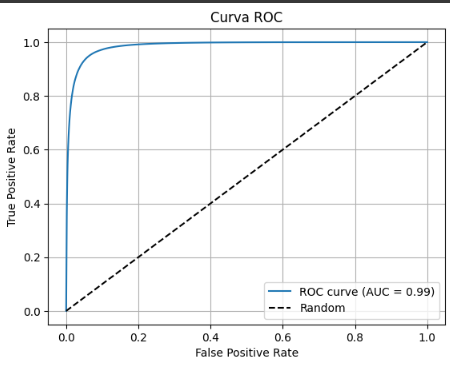
\includegraphics[width=0.6\linewidth]{ROC.png}
    \caption{Curva ROC del modelo final mostrando un AUC de 0.99. La curva se aproxima al punto óptimo (0,1), indicando un rendimiento excelente. La línea punteada representa el rendimiento aleatorio (AUC = 0.50).}
    \label{fig:roc_curve}
\end{figure}

\textbf{Resultado Obtenido: AUC-ROC = 0.99}

Este valor de AUC-ROC de 0.99 indica un rendimiento excelente del modelo, confirmando su capacidad superior para distinguir entre estrellas y galaxias. Un AUC cercano a 1.0 demuestra que el modelo mantiene alta sensibilidad (detección correcta de galaxias) mientras minimiza los falsos positivos (estrellas clasificadas incorrectamente como galaxias).

\newpage

\section{Conclusión}

\subsection{Conclusiones del Proyecto}

Este proyecto logró desarrollar exitosamente un sistema de clasificación automática para distinguir entre estrellas y galaxias utilizando datos del Sloan Digital Sky Survey (SDSS). Los resultados obtenidos superaron las expectativas iniciales y demuestran la viabilidad de aplicar técnicas de machine learning a problemas de clasificación.

\textbf{Resultados Principales:}
\begin{itemize}
    \item \textbf{Accuracy final: 94.24\%} en el dataset de test, superando el objetivo inicial de >90\%
    \item \textbf{Modelo implementado:} Regresión Logística con regularización L1 optimizada, que proporciona excelente capacidad de generalización y eficiencia computacional
    \item \textbf{Pipeline robusto:} Desarrollo de un sistema de preprocesado especializado que maneja transformaciones logarítmicas y escalado robusto específico para datos astronómicos
    \item \textbf{Selección de características:} Identificación de 13 variables discriminativas clave que capturan las diferencias físicas fundamentales entre objetos puntuales y extendidos
\end{itemize}

\textbf{Impacto Práctico:}
El modelo final ofrece una solución eficiente para el procesamiento automático de millones de objetos astronómicos, reduciendo significativamente el tiempo y recursos necesarios para la clasificación manual.

\subsection{Problemas Enfrentados y Soluciones}

Durante el desarrollo del proyecto se encontraron varios desafíos técnicos que requirieron soluciones específicas:

\textbf{1. Tamaño Masivo del Dataset (4 millones de observaciones):}
\begin{itemize}
    \item \textbf{Problema:} Limitaciones de memoria y tiempo de procesamiento extremadamente largos
    \item \textbf{Solución:} Implementación de muestreo estratificado (100,000 muestras) para desarrollo y optimización, manteniendo el balance de clases. Uso del dataset completo solo para entrenamiento final
\end{itemize}

\textbf{2. Alta Dimensionalidad (51 variables originales):}
\begin{itemize}
    \item \textbf{Problema:} Riesgo de sobreajuste con la dimensionalidad y presencia de variables redundantes o irrelevantes
    \item \textbf{Solución:} Análisis de correlaciones y selección basada en conocimiento de las variables, reduciendo a 13 variables discriminativas clave
\end{itemize}

\textbf{3. Necesidad de Regularización Adecuada:}
\begin{itemize}
    \item \textbf{Problema:} Riesgo de sobreajuste debido a la alta dimensionalidad y complejidad de las relaciones en datos astronómicos
    \item \textbf{Solución:} Implementación de regularización L1 en la Regresión Logística, que proporciona selección automática de características y previene el sobreajuste
\end{itemize}

\textbf{4. Complejidad de Variables Astronómicas:}
\begin{itemize}
    \item \textbf{Problema:} Dificultad para interpretar parámetros técnicos como radios petrosianos, parámetros de Stokes y diferencias entre magnitudes PSF vs modelo
    \item \textbf{Solución:} Investigación de literatura astronómica y análisis exploratorio detallado para comprender el significado físico de cada variable
\end{itemize}

\textbf{5. Distribuciones Altamente Sesgadas:}
\begin{itemize}
    \item \textbf{Problema:} Variables con distribuciones log-normales extremas y concentración cerca de cero (especialmente flujos y parámetros de Stokes)
    \item \textbf{Solución:} Implementación de transformaciones logarítmicas (log1p) y uso de RobustScaler para manejar outliers astronómicos legítimos sin perder información valiosa
\end{itemize}

\textbf{Reflexión Personal:}
Este proyecto evidenció la importancia de combinar conocimiento de las variables con técnicas de machine learning robustas. La principal lección aprendida fue que un preprocesado especializado y una regularización adecuada son fundamentales para obtener modelos que generalicen bien en datos reales. El balance entre interpretabilidad, eficiencia computacional y precisión resultó ser crucial para desarrollar una solución práctica y escalable.

\newpage

\addcontentsline{toc}{section}{Bibliografía}
\begin{thebibliography}{9}

\bibitem{sklearn_lr}
Scikit-learn developers. (2025). \textit{sklearn.linear\_model.LogisticRegression}. 
Disponible en: \url{https://scikit-learn.org/stable/modules/generated/sklearn.linear_model.LogisticRegression.html}

\bibitem{kaggle_dataset}
Hari31416. (2024). \textit{CelestialClassify - Stellar and Galactic Classification Dataset}. Kaggle. 
Disponible en: \url{https://www.kaggle.com/datasets/hari31416/celestialclassify}

\bibitem{colab_notebook}
De Alba, J.P. (2025). \textit{Clasificación Binaria de Estrellas y Galaxias - Notebook de Implementación}. Google Colab. 
Disponible en: \url{https://colab.research.google.com/drive/1Z7cGOq95QmInkWO31x2LaOZ4O5ohhJIZ?usp=sharing}

\bibitem{sklearn_robustscaler}
Scikit-learn developers. (2025). \textit{sklearn.preprocessing.RobustScaler}. 
Disponible en: \url{https://scikit-learn.org/stable/modules/generated/sklearn.preprocessing.RobustScaler.html}

\bibitem{sklearn_simpleimputer}
Scikit-learn developers. (2025). \textit{sklearn.impute.SimpleImputer}. 
Disponible en: \url{https://scikit-learn.org/stable/modules/generated/sklearn.impute.SimpleImputer.html}

\bibitem{accuracy_metric}
CloudFactory. (2024). \textit{Accuracy - Machine Learning Metrics}. CloudFactory Wiki. 
Disponible en: \url{https://wiki.cloudfactory.com/docs/mp-wiki/metrics/accuracy}

\bibitem{recall_metric}
CloudFactory. (2024). \textit{Recall - Machine Learning Metrics}. CloudFactory Wiki. 
Disponible en: \url{https://wiki.cloudfactory.com/docs/mp-wiki/metrics/recall}

\bibitem{fscore_metric}
CloudFactory. (2024). \textit{F-Beta Score - Machine Learning Metrics}. CloudFactory Wiki. 
Disponible en: \url{https://wiki.cloudfactory.com/docs/mp-wiki/metrics/f-beta-score}

\bibitem{precision_metric}
CloudFactory. (2024). \textit{Precision - Machine Learning Metrics}. CloudFactory Wiki. 
Disponible en: \url{https://wiki.cloudfactory.com/docs/mp-wiki/metrics/precision}

\bibitem{roc_metric}
CloudFactory. (2024). \textit{Precision-Recall Curve and AUC-PR - Machine Learning Metrics}. CloudFactory Wiki. 
Disponible en: \url{https://wiki.cloudfactory.com/docs/mp-wiki/metrics/precision-recall-curve-and-auc-pr}

\bibitem{cohen_kappa}
Scikit-learn developers. (2025). \textit{sklearn.metrics.cohen\_kappa\_score}. 
Disponible en: \url{https://scikit-learn.org/stable/modules/generated/sklearn.metrics.cohen_kappa_score.html}

\bibitem{roc_analysis}
Scikit-learn developers. (2025). \textit{sklearn.metrics.roc\_curve}. 
Disponible en: \url{https://scikit-learn.org/stable/modules/generated/sklearn.metrics.roc_curve.html}

\bibitem{chi2_test}
Scikit-learn developers. (2025). \textit{sklearn.feature\_selection.chi2}. 
Disponible en: \url{https://scikit-learn.org/stable/modules/generated/sklearn.feature_selection.chi2.html}

\end{thebibliography}

\end{document}
